\documentclass{article}
\usepackage[final]{nips_2017}
\usepackage{polski}
\usepackage[utf8]{inputenc}    % allow utf-8 input
\usepackage[T1]{fontenc}       % use 8-bit T1 fonts
\usepackage{hyperref}          % hyperlinks
\usepackage{url}               % simple URL typesetting
\usepackage{booktabs}          % professional-quality tables
\usepackage{amsfonts}          % blackboard math symbols
\usepackage{nicefrac}          % compact symbols for 1/2, etc.
\usepackage{microtype}         % microtypography
\usepackage[section]{placeins} % figures kept in sections
\usepackage{graphicx}          % images
\graphicspath{ {./img/} }
\usepackage{multirow}

\title{  Perceptron prosty i Adaline\\Sieci Neuronowe 2020 }

\author{
  Jakub Ciszek \\
  238035\\
}

\begin{document}

\maketitle

\newpage
\tableofcontents
\newpage

Cały kod wykorzystany w zadaniu znajduje się pod adresem: \url{https://github.com/Greenpp/sieci-neuronowe-pwr-2020}

\section{Opis badań}
\subsection{Plan eksperymentów}

Wszystkie eksperymenty zostały przeprowadzone 100 razy. Losowość przy inicjalizacji wag oraz generacji danych nie została narzucona żadnym ziarnem. Podczas badań przyjęto górną granicę 1000 epok, po przekroczeniu której, przy pierwszych 6 wyuczeniach, model zostawał klasyfikowany jako niezdolny do wyuczenia. Zgodnie z instrukcją zostały przeprowadzone następujące badania:
\begin{itemize}
	\item Wpływ wartości progu theta na szybkość uczenia Perceptronu
	\item Wpływ zakresu inicjalizacji wag na szybkość uczenia Perceptronu
	\item Wpływ wartości współczynnika uczenia alpha na szybkość uczenia Perceptronu
	\item Wpływ funkcji aktywacyjnej (unipolarna, bipolarna) na szybkość uczenia Perceptronu
	\item Wpływ zakresu inicjalizacji wag na szybkość uczenia Adaline
	\item Wpływ wartości współczynnika uczenia alpha na szybkość uczenia Adaline
	\item Wpływ przyjętego dopuszczalnego błędu na wynik uczenia w Adaline
	\item Porównanie Perceptronu i Adaline
\end{itemize}

\subsection{Charakterystyka zbiorów danych}

Dane użyte w zadaniu są reprezentacją logicznej funkcji AND

\begin{table}[h]
	\caption{Wartości funkcji AND}
	\label{tabela-and}
	\centering
	\begin{tabular}{llc}
		\toprule
		\(a\) & \(b\) & \(a \land b\) \\
		\midrule
		0     & 0     & 0             \\
		0     & 1     & 0             \\
		1     & 1     & 1             \\
		1     & 0     & 0             \\
		\bottomrule
	\end{tabular}
\end{table}

W trakcie eksperymentów wykorzystano 2 zbiory, uczący oraz walidujący.
\begin{itemize}
	\item Zbiór uczący: 4 podstawowe wzorce oraz 4-krotna kopia każdego z nich z przesuniętymi wartościami wejściowymi o \(\pm\ $-0.01 -- 0.01$\)
	\item Zbiór walidujący: 4 podstawowe wzorce
\end{itemize}

\newpage
\section{Eksperymenty}

\subsection{Wpływ wartości progu theta na szybkość uczenia Perceptronu}
\subsubsection*{Założenia}
\begin{table}[h]
	\caption{Stałe dla eksperymentu 1}
	\label{tabela-const-1}
	\centering
	\begin{tabular}{ll}
		\toprule
		Parametr               & Wartość         \\
		\midrule
		Bias                   & Nie               \\
		Zakres wag             & \($-0.2 -- 0.2$\) \\
		Współczynnik uczenia & 0.01              \\
		\bottomrule
	\end{tabular}
\end{table}

Zmienną w tym eksperymencie była wartość theta dla funkcji aktywacji. Przyjmowała wartości ze zbioru \(\{$-1, -0.5, 0, 0.5, 1$\}\)
\subsubsection*{Przebieg}

Podczas eksperymentu model został zainicjalizowany 100 razy dla każdej z badanych wartości oraz wyuczony, uzyskane wyniki zostały zapisane w postaci pliku .plk do dalszej analizy. Badanie przeprowadzono dla funkcji aktywacyjnej unipolarnej jak i bipolarnej. Przebadane zostały też wartości dynamicznego progu.

\subsubsection*{Wyniki}
\begin{figure}[h]
	\centering
	\caption{Zależność szybkości uczenia od parametru theta}
	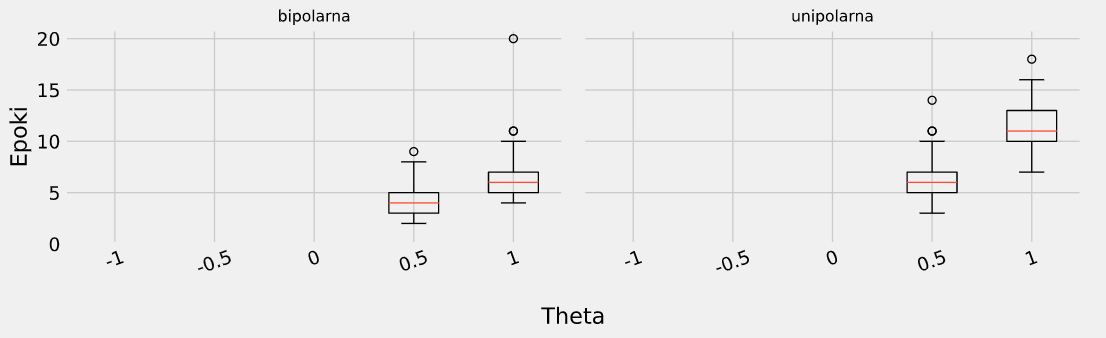
\includegraphics[width=\textwidth]{per_theta.png}
	\label{fig:res11}
\end{figure}

\begin{table}[h]
	\caption{Średnia ilość epok potrzebna do wyuczenia w zależności od parametru theta}
	\label{tabela-res-11}
	\centering
	\begin{tabular}{rrr}
		\toprule
		\multirow{2}{*}{Theta}   & \multicolumn{2}{c}{Epoki} \\
		     & bipolarna & unipolarna \\
		\midrule
		-1.0 & -         & -          \\
		-0.5 & -         & -          \\
		0.0  & -         & -          \\
		0.5  & 3.85      & 6.46       \\
		1.0  & 6.4       & 11.46      \\
		\bottomrule
	\end{tabular}
\end{table}

\begin{figure}[h]
	\centering
	\caption{Wartości dynamicznego progu}
	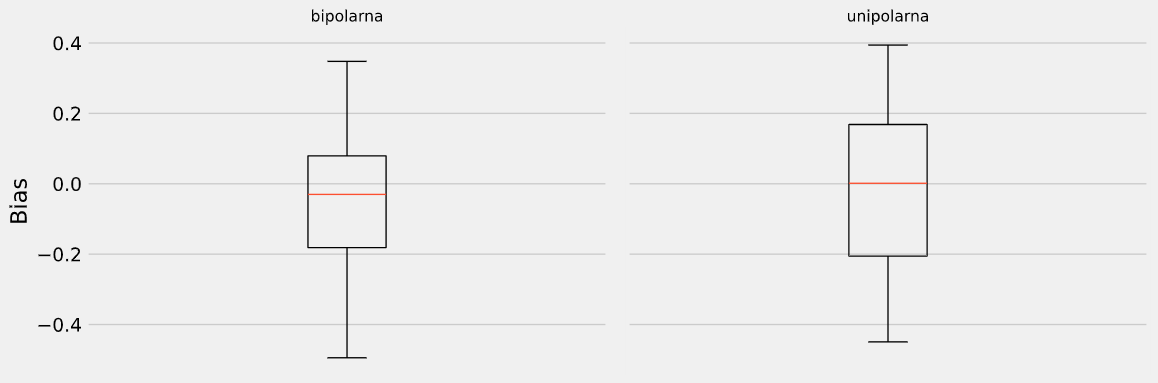
\includegraphics[width=\textwidth]{per_bias.png}
	\label{fig:res12}
\end{figure}

\begin{table}[h]
	\caption{Średnia wartość progu po wyuczeniu (- bias) }
	\label{tabela-res-12}
	\centering
	\begin{tabular}{lrr}
		\toprule
		Aktywacja  & Próg  \\
		\midrule
		bipolarna  & 0.0507 \\
		unipolarna & 0.0230 \\
		\bottomrule
	\end{tabular}
\end{table}

\subsubsection*{Wnioski}

% TODO

\newpage
\subsection{Wpływ zakresu inicjalizacji wag na szybkość uczenia Perceptronu}
\subsubsection*{Założenia}
\begin{table}[h]
	\caption{Stałe dla eksperymentu 2}
	\label{tabela-const-2}
	\centering
	\begin{tabular}{ll}
		\toprule
		Parametr               & Wartość \\
		\midrule
		Bias                   & Tak       \\
		Theta                  & 0         \\
		Współczynnik uczenia & 0.01      \\
		\bottomrule
	\end{tabular}
\end{table}

Zmienną w tym eksperymencie była wartość początkowego zakresu wag. Przyjmowała wartości ze zbioru \(\{$0, -0.1 - 0.1, -0.2 - 0.2, -0.5 - 0.5, -0.8 - 0.8, -1 - 1$\}\)
\subsubsection*{Przebieg}

Podczas eksperymentu model został zainicjalizowany 100 razy dla każdej z badanych wartości oraz wyuczony, uzyskane wyniki zostały zapisane w postaci pliku .plk do dalszej analizy. Badanie przeprowadzono dla funkcji aktywacyjnej unipolarnej jak i bipolarnej.

\subsubsection*{Wyniki}
\begin{figure}[h]
	\centering
	\caption{Zależność szybkości uczenia od początkowego zakresu wag}
	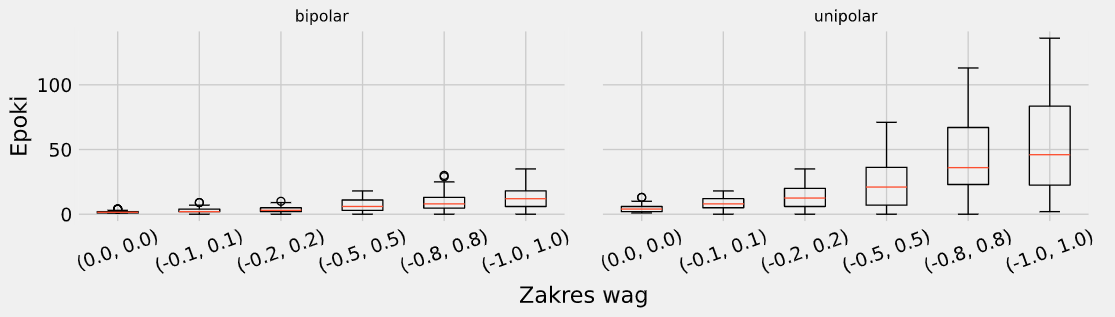
\includegraphics[width=\textwidth]{per_w.png}
	\label{fig:res2}
\end{figure}

\begin{table}[h]
	\caption{Średnia ilość epok potrzebna do wyuczenia w zależności od początkowego zakresu wag}
	\label{tabela-res-2}
	\centering
	\begin{tabular}{rrr}
		\toprule
		\multirow{2}{*}{Zakres wag}   & \multicolumn{2}{c}{Epoki} \\
		                  & bipolarna & unipolarna \\
		\midrule
		0                 & 2.07      & 4.31       \\
		\($-0.1 -- 0.1$\) & 2.99      & 9.03       \\
		\($-0.2 -- 0.2$\) & 3.88      & 13.64      \\
		\($-0.5 -- 0.5$\) & 6.99      & 23.53      \\
		\($-0.8 -- 0.8$\) & 10.59     & 40.50      \\
		\($-1.0 -- 1.0$\) & 12.26     & 47.52      \\
		\bottomrule
	\end{tabular}
\end{table}

\subsubsection*{Wnioski}

% TODO

\newpage
\subsection{Wpływ wartości współczynnika uczenia alpha na szybkość uczenia Perceptronu}
\subsubsection*{Założenia}

\begin{table}[h]
	\caption{Stałe dla eksperymentu 3}
	\label{tabela-const-3}
	\centering
	\begin{tabular}{ll}
		\toprule
		Parametr   & Wartość         \\
		\midrule
		Bias       & Tak               \\
		Theta      & 0                 \\
		Zakres wag & \($-0.5 -- 0.5$\) \\
		\bottomrule
	\end{tabular}
\end{table}

Zmienną w tym eksperymencie była wartość współczynnika uczenia. Przyjmowała wartości ze zbioru \(\{$0.0001, 0.001, 0.01, 0.1, 1$\}\)

\subsubsection*{Przebieg}

Podczas eksperymentu model został zainicjalizowany 100 razy dla każdej z badanych wartości oraz wyuczony, uzyskane wyniki zostały zapisane w postaci pliku .plk do dalszej analizy. Badanie przeprowadzono dla funkcji aktywacyjnej unipolarnej jak i bipolarnej.

\subsubsection*{Wyniki}

\begin{figure}[h]
	\centering
	\caption{Zależność szybkości uczenia od parametru alpha}
	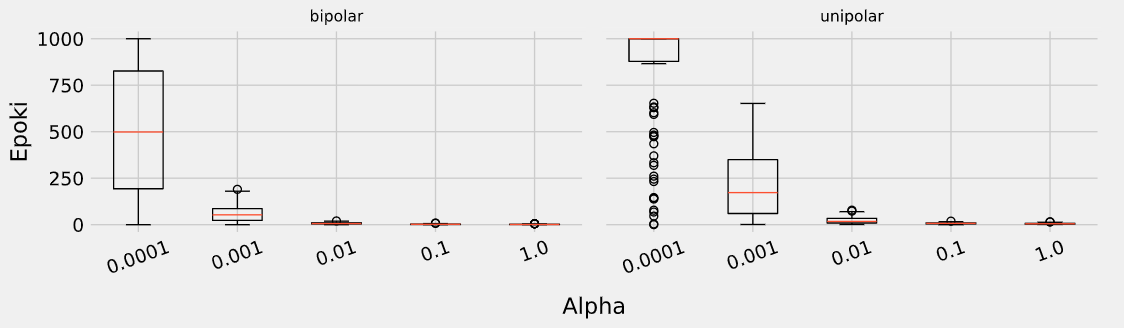
\includegraphics[width=\textwidth]{per_alpha.png}
	\label{fig:res3}
\end{figure}

\begin{table}[h]
	\caption{Średnia ilość epok potrzebna do wyuczenia w zależności od parametru alpha}
	\label{tabela-res-3}
	\centering
	\begin{tabular}{rrr}
		\toprule
		\multirow{2}{*}{Alpha}   & \multicolumn{2}{c}{Epoki} \\
		       & bipolarna & unipolarna \\
		\midrule
		0.0001 & 515.41    & 848.95     \\
		0.0010 & 53.58     & 216.23     \\
		0.0100 & 7.77      & 23.15      \\
		0.1000 & 2.17      & 7.03       \\
		1.0000 & 1.75      & 5.41       \\
		\bottomrule
	\end{tabular}
\end{table}

\subsubsection*{Wnioski}

% TODO

\newpage
\subsection{Wpływ funkcji aktywacyjnej (unipolarna, bipolarna) na szybkość uczenia Perceptronu}
\subsubsection*{Wnioski}

\newpage
\subsection{Wpływ zakresu inicjalizacji wag na szybkość uczenia Adaline}
\subsubsection*{Założenia}
\begin{table}[h]
	\caption{Stałe dla eksperymentu 5}
	\label{tabela-const-5}
	\centering
	\begin{tabular}{ll}
		\toprule
		Parametr               & Wartość \\
		\midrule
		Bias                   & Tak       \\
		Theta                  & 0         \\
		Współczynnik uczenia & 0.01      \\
		Epsilon                & 0.2       \\
		\bottomrule
	\end{tabular}
\end{table}

Zmienną w tym eksperymencie była wartość początkowego zakresu wag. Przyjmowała wartości ze zbioru \(\{$0, -0.1 - 0.1, -0.2 - 0.2, -0.5 - 0.5, -0.8 - 0.8, -1 - 1$\}\)

\subsubsection*{Przebieg}

Podczas eksperymentu model został zainicjalizowany 100 razy dla każdej z badanych wartości oraz wyuczony, uzyskane wyniki zostały zapisane w postaci pliku .plk do dalszej analizy.
\subsubsection*{Wyniki}

\begin{figure}[h]
	\centering
	\caption{Zależność szybkości uczenia od początkowego zakresu wag}
	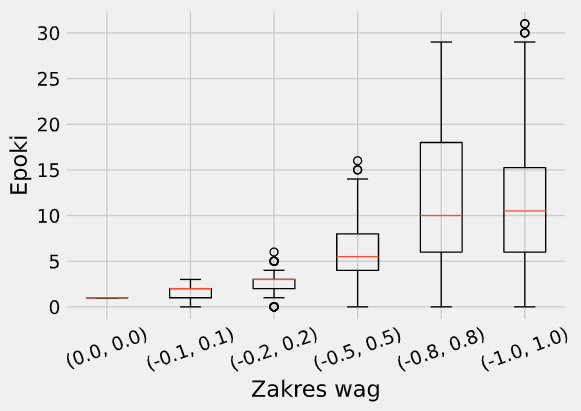
\includegraphics[width=.5\textwidth]{ada_w.png}
	\label{fig:res5}
\end{figure}

\begin{table}[h]
	\caption{Średnia ilość epok potrzebna do wyuczenia w zależności od początkowego zakresu wag}
	\label{tabela-res-5}
	\centering
	\begin{tabular}{rrr}
		\toprule
		Zakres wag        & Epoki \\
		\midrule
		0                 & 1.00  \\
		\($-0.1 -- 0.1$\) & 1.52  \\
		\($-0.2 -- 0.2$\) & 2.55  \\
		\($-0.5 -- 0.5$\) & 6.51  \\
		\($-0.8 -- 0.8$\) & 9.70  \\
		\($-1.0 -- 1.0$\) & 11.97 \\
		\bottomrule
	\end{tabular}
\end{table}

\subsubsection*{Wnioski}

\newpage
\subsection{Wpływ wartości współczynnika uczenia alpha na szybkość uczenia Adaline}
\subsubsection*{Założenia}

\begin{table}[h]
	\caption{Stałe dla eksperymentu 6}
	\label{tabela-const-6}
	\centering
	\begin{tabular}{ll}
		\toprule
		Parametr   & Wartość         \\
		\midrule
		Bias       & Tak               \\
		Theta      & 0                 \\
		Zakres wag & \($-0.5 -- 0.5$\) \\
		Epsilon    & 0.2               \\
		\bottomrule
	\end{tabular}
\end{table}

Zmienną w tym eksperymencie była wartość współczynnika uczenia. Przyjmowała wartości ze zbioru \(\{$0.0001, 0.001, 0.01, 0.1, 1$\}\)

\subsubsection*{Przebieg}

Podczas eksperymentu model został zainicjalizowany 100 razy dla każdej z badanych wartości oraz wyuczony, uzyskane wyniki zostały zapisane w postaci pliku .plk do dalszej analizy.

\subsubsection*{Wyniki}

\begin{figure}[h]
	\centering
	\caption{Zależność szybkości uczenia od parametru alpha}
	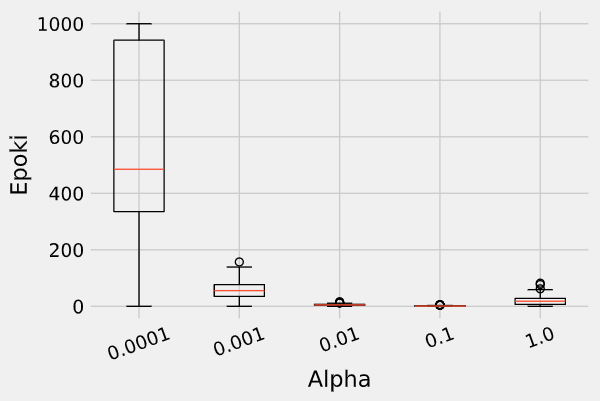
\includegraphics[width=.5\textwidth]{ada_alpha.png}
	\label{fig:res6}
\end{figure}

\begin{table}[h]
	\caption{Średnia ilość epok potrzebna do wyuczenia w zależności od parametru alpha}
	\label{tabela-res-6}
	\centering
	\begin{tabular}{rrr}
		\toprule
		Alpha  & Epoki  \\
		\midrule
		0.0001 & 553.30 \\
		0.0010 & 55.47  \\
		0.0100 & 5.43   \\
		0.1000 & 1.68   \\
		1.0000 & 21.41  \\
		\bottomrule
	\end{tabular}
\end{table}

\subsubsection*{Wnioski}

\newpage
\subsection{Wpływ przyjętego dopuszczalnego błędu na wynik uczenia w Adaline}
\subsubsection*{Założenia}
\begin{table}[h]
	\caption{Stałe dla eksperymentu 7}
	\label{tabela-const-7}
	\centering
	\begin{tabular}{ll}
		\toprule
		Parametr               & Wartość         \\
		\midrule
		Bias                   & Tak               \\
		Theta                  & 0                 \\
		Zakres wag             & \($-0.5 -- 0.5$\) \\
		Współczynnik uczenia & 0.01              \\
		Epsilon                & 0                 \\
		\bottomrule
	\end{tabular}
\end{table}
\subsubsection*{Przebieg}

Podczas eksperymentu model został zainicjalizowany 100 raz, po czym zostało sprawdzone zachowanie błędu. uzyskane wyniki zostały zapisane w postaci pliku .plk do dalszej analizy.

\subsubsection*{Wyniki}

\begin{figure}[h]
	\centering
	\caption{Zachowanie błędu w trakcie uczenia Adaline}
	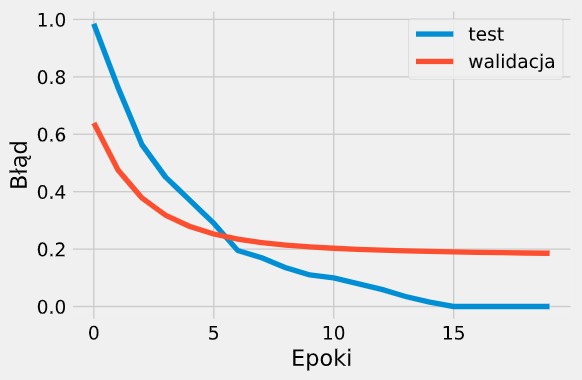
\includegraphics[width=.5\textwidth]{ada_epsilon.png}
	\label{fig:res7}
\end{figure}

Minimalna zaobserwowana wartość błędu walidacji: \($0.1307$\)

\subsubsection*{Wnioski}

Uzyskane wyniki zostały ograniczone do 20 epok z powodu zerowego błędu testowego podczas dalszego uczenia.

\newpage
\subsection{Porównanie Perceptronu i Adaline}
\subsubsection*{Założenia}
\subsubsection*{Przebieg}
\subsubsection*{Wyniki}

\begin{figure}[h]
	\centering
	\caption{Porównanie szybkości uczenia Perceptronu i Adaline w zależności od początkowego zakresu wag}
	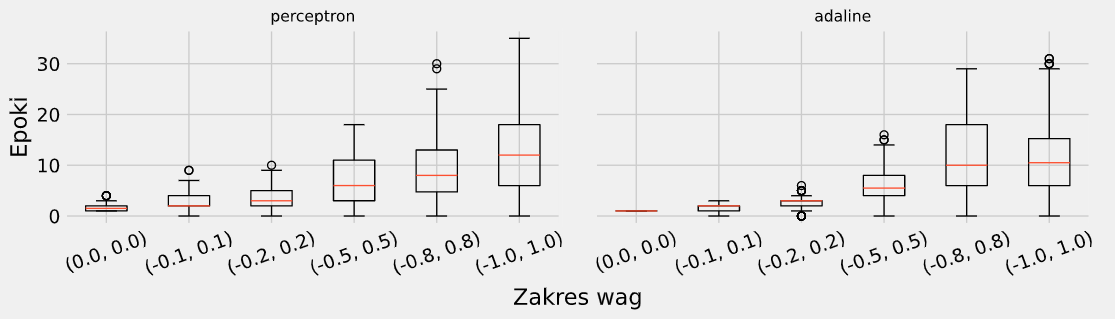
\includegraphics[width=\textwidth]{ada_per_w.png}
	\label{fig:res81}
\end{figure}

\begin{table}[h]
	\caption{Porównanie średniej ilości epok potrzebnych do wyuczenia Perceptronu i Adaline w zależności od początkowego zakresu wag}
	\label{tabela-res-81}
	\centering
	\begin{tabular}{rrr}
		\toprule
		\multirow{2}{*}{Zakres wag}   & \multicolumn{2}{c}{Epoki} \\
		                  & Perceptron & Adaline        \\
		\midrule
		0                 & 2.07       & \textbf{1.00}  \\
		\($-0.1 -- 0.1$\) & 2.99       & \textbf{1.52}  \\
		\($-0.2 -- 0.2$\) & 3.88       & \textbf{2.55}  \\
		\($-0.5 -- 0.5$\) & 6.99       & \textbf{6.51}  \\
		\($-0.8 -- 0.8$\) & 10.59      & \textbf{9.70}  \\
		\($-1.0 -- 1.0$\) & 12.26      & \textbf{11.97} \\
		\bottomrule
	\end{tabular}
\end{table}


\begin{figure}[h]
	\centering
	\caption{Porównanie szybkości uczenia Perceptronu i Adaline w zależności od parametru alpha}
	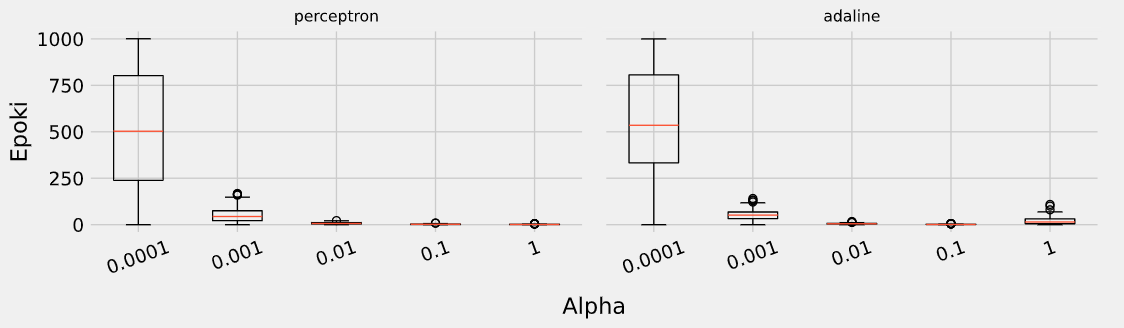
\includegraphics[width=\textwidth]{ada_per_alpha.png}
	\label{fig:res82}
\end{figure}

\begin{table}[h]
	\caption{Porównanie średniej ilości epok potrzebnych do wyuczenia Perceptronu i Adaline w zależności od parametru alpha}
	\label{tabela-res-82}
	\centering
	\begin{tabular}{rrr}
		\toprule
		\multirow{2}{*}{Alpha}   & \multicolumn{2}{c}{Epoki} \\
		       & Perceptron      & Adaline       \\
		\midrule
		0.0001 & \textbf{515.41} & 553.30        \\
		0.0010 & \textbf{53.58}  & 55.47         \\
		0.0100 & 7.77            & \textbf{5.43} \\
		0.1000 & 2.17            & \textbf{1.68} \\
		1.0000 & \textbf{1.75}   & 21.41         \\
		\bottomrule
	\end{tabular}
\end{table}

\subsubsection*{Wnioski}

\newpage
\section{Wnioski}

\end{document}